\section{開発内容}
%開発内容(項目)と各開発結果の詳細な説明
%本プロジェクトの開発内容について,開発機能の項目毎に,あるいは設計・実装・テスト・評価等の項目に分割し,どのような開発(or  取り組み)をしたのかとその結果などを図・表やサンプル画面なども付加して『詳細に記述』してください.
%この「4. 開発内容」で本プロジェクトの開発内容がわかり易く,かつ具体的に記述されていない場合は,成果報告書の修正をしてもらう場合があります.

本プロジェクトは,視覚(光学的)情報を適切な方法で音響化することにより,聴覚による空間知覚を可能にするデバイス「Sight」を開発することを目標とするものである.
九ヶ月間のプロジェクト実施期間を通じて我々は,「Sight」装着状態でより高度な空間知覚タスクの実行を可能にすべく,ヒトの視聴覚の特性に関する調査・検討を重ねつつ複数の視聴覚変換手法を開発した.
本セクションでは,各段階のバージョンにおいて提案された変換手法について,その技術的詳細と上記目標に対する実現度の評価を述べる.

いずれのバージョンにおいても,「Sight」は搭載した光学的センサからの入力(視覚情報)をパラメータ化し,このパラメータを用いてソフトウェアシンセサイザにより音響を合成するという処理のフローを採用する.
従って,視覚情報のパラメータ化,音響のパラメータ表現,および両者のパラメータの対応付けという三種類の変換の組み合わせにより入出力が対応させられることとなる.
以下,第一の変換にあたる「外界の認識」と第二・第三の変換にあたる「音響合成戦略」の二部に分けて各提案手法を詳説する.

また,本プロジェクトでは視聴覚変換手法のソフトウェア実装の他,装着用のハードウェアもデザイン・製作した.
本セクションでは「Sight」デバイスのハードウェアについても開発の経緯及び工夫点を解説する.


\subsection{外界の認識}

視覚的な外界の認識,すなわち光学的センサ入力の分析によるパラメータ化方式は,「Sight」システムが実現する「視覚」体験において提供される情報の内容および分量を規定する支配的要因である.
プロジェクト開始時には我々は,耳による直接的な目の代替を目指し,比較的低次の画像特徴量を多数抽出することで,通常目を通して受容するすべての視覚情報をパラメータ化することを試みた(バージョン1).
次いで,物体把握に必要な視覚特徴量の適切な抽象化レベルを探求すべく,一般物体認識用深層ニューラルネットワークの中間層をパラメータ生成に利用する新手法を考案し,性能評価を行った(バージョン2).

上記2バージョンを用いた実験の実施により,画像特徴量に基づくパラメータ化が学習の汎化に困難があると判明したため,周囲の空間構造という抽象化された情報の知覚を目標として再設定した.
まず,イルカやコウモリをはじめ多くの動物がエコーロケーションと呼ばれる反響を利用したアクティブセンシングによって,障害物や他の動物の存在を知覚する視覚的機能を実現している事例を参考として,深度センサを用いて周囲の物体との距離を単純に聴覚化することを試みた(バージョン3).
次いで,生態光学の理論に基づき行動可能性の把握に基礎を置く視覚の機能的再定義を図り,支持平面や障害物といった空間の基礎的な意味構造分析にもとづく,認知的に自然と考えられる高次のパラメータ化手法を開発した(バージョン4).

\subsubsection{バージョン1: 低次の特徴点・局所特徴量(SURF)の分布}

\heading{アイディア}
ヒトを含む霊長類の視覚は,網膜で捉えた最低次の光学的刺激の配列を一次視覚野(V1),二次視覚野(V2)等の脳領域で順次抽象化していく過程としてモデル化されている.
例えば一次視覚野のニューロンは網膜上の点との一対一対応(レチノトピー)を保っていることが知られており,入力に対してフィルタ処理に相当する応答が行われることで,空間的パターンや運動の知覚に必要な情報が抽出される.
また,近年の研究では,外部センサにより磁気刺激をマウスの一次視覚野に入力することで知覚代替(Sensory Substitution)が可能であること[Norimoto and Ikegaya, 2015]や,
視覚障害者がクリック音によるエコーロケーションを行う際に脳の視覚関連領域が活発に活動していること
[?]が知られており,
侵襲的処理や長期間の学習により,聴覚刺激など様々な入力を視覚野で処理できるようになる可塑性を脳が備えていると考えられている.

「Sight」最初期バージョンでは,こうした神経系でのボトムアップな情報処理及び可塑性に注目し,音響にエンコードされ耳へと入力される空間情報が視覚処理経路に直接バイパスされることによって,聴取による視覚が実現されることを目指した.
しかし,ヒトの聴覚の解像度(帯域幅)は,多数の視細胞からの入力を並列処理する視覚に比べて著しく小さく,光学刺激の空間パターンを単純に音響にエンコードしても,パターン認識などの抽象化に耐える情報量を聴取できるとは期待しづらい.
そこで,低次視覚野における情報の抽象化をソフトウェア的に模倣することで,神経系における情報処理との親和性を確保しつつ音響に変換される情報量の削減を図った.

\heading{実装}
入力デバイスとしては,目を模倣して一般的なRGB画像を出力するウェブカメラを用いる.
低次視覚野(V1)で行われるフィルタ処理とコンピュータビジョンにおける画像の局所特徴量計算との類似性に注目し,RGBカメラからの入力画像に対して特徴点検出器によって抽出された特徴点およびそれらの特徴ベクトルによって,入力の抽象化された表現とする.
今回の実装では,特徴点抽出アルゴリズムとしてはOpenCV 2.4実装のSURF(Speeded up robust features)を採用し,サイズ上位30個までの特徴点を音響生成に利用した.
各特徴点は64次元の特徴ベクトルで表現されるが,この次元をさらに削減するために,室内環境で収集した10,000個の特徴ベクトルに対して主成分分析を行い,上位成分のみを採用することで10次元のベクトル表現を得た.
10次元で表現された特徴ベクトルは,近傍の平均色および画像上の座標を加えて1つの音源に対応するオブジェクトとして保存され,音響生成ルーチンへと送信される.

\heading{評価}
本手法に基づく「Sight」を利用した評価・感想については音響変換の節で詳しく述べるため,本節では画像認識および特徴量に関する客観的な評価を概説する.

まず,一般的傾向としてSURF特徴点は画像上のエッジや角にあたる部分に検出されるため,滑らかな平面や壁面の画像を入力とした場合は少数で一様な特徴点が得られ,複雑な画像を入力とした場合は多数かつ雑多な成分分布を持つベクトル群が得られた.
このように視野の大域的特徴に関して特徴量分布が強い定性的相関を示すため,視野内の大規模な構造の変化(例えば壁面に顔を向けた場合,屋内外の変化など,平坦な地面と複雑な立ち木など)に対しては概ね鋭敏である.
一方,特徴点の検出位置は不安定性が強く,入力動画の連続したフレームでも僅かな頭部の動きや物体の移動にともなって,大きく上位特徴点の位置分布がずれる傾向が見られた.
これにより,特定の物体(机の上に置いたリンゴなど)に由来する特徴点であっても検出位置(リンゴのヘタ部分か側面か,など)によってベクトルが大幅に変動するので,物体の同一性を特徴ベクトルから推測するのは難しいことが分かった.

主成分分析による次元削減アルゴリズムに関しては,似た特徴点を大まかに似たベクトルとして変換する傾向が確認できた.
例えば,机の同一の縁上に検出された複数の特徴点は,いずれも似た局所的外見を目視できるが,これは次元削減後のベクトルの類似性にも反映されている.
一方,上述の通りある物体に関して様々な箇所の特徴点がフレームごとランダムに検出されるため,単一の物体上であっても雑多なベクトル群が出力される.
従って,直接ベクトルの分布を観察しても,物体を特徴点群のベクトルによって識別することは著しく難しいことが判明した.

本手法によって大まかに「何かがあるか」,「それは複雑な外見をしているか」,「それはどちらに動いているか」といった情報を捉えることは可能であるが,主に特徴点検出位置の不安定性および,特徴ベクトルの非特異性(様々な物体から似たベクトルが得られる)により,どのような状況であるかを知らせる情報は著しく欠落するという結論が得た.
検出する特徴点の個数を増やすことで検出位置の不安定性には対処が可能であるが,この場合聴取すべき情報量が増大するので認知的負荷は大きく増大する.
このように,低次の局所特徴量を用いるアプローチでは大幅な次元削減を行ったとしても,シーンを把握するために聴取すべき情報量は大きくなりすぎる傾向があるという知見から,以降のバージョンではより抽象度を高めたデータ分析によりシーン特異性を高めるアプローチに移行した.

ToDo: echo location引用
ToDo: Figureを入れる


\subsubsection{バージョン2: 一般物体認識のDNNを用いたモデル}

\heading{アイディア}
一般物体認識の領域で非常に良好な成績を納めているDeep Neural Networkというモデルがある.
これは既存のフィードフォワード型のニューラルネットワークを多層化したものであるが,
シンプルに多層化するとバックプロパゲーション学習の効果が薄れてしまうという欠点を克服するため,
初期値の決定に関してオートエンコーダなど新しい特徴抽出の仕組みを取り入れたものである.
このような既存のモデルは,ILSVRCという一般物体認識の性能コンテストに
応募されたたくさんのモデルおよびそれを解説した論文に詳しく記されている.

このようなDNNの入力層に画像を与えてフィードフォワード計算を行うと,
ニューラルネットワークの最終層の出力には
分類の結果に関する情報が生成される.
ILSVRCでは1000カテゴリの物体認識を行うので,この出力は1000次元である.
最初は,この分類カテゴリ情報を元に音に変換する実装を行ったが,
この方式には2つの欠点があった.
1つは「学習したカテゴリ以外の者に拡張することができない」というものである.
見たことのないものは,角度や見え方に寄って,似た複数のもののカテゴリ間で振動したり
全く見当違いのカテゴリとして認識されたりしてしまう.
もう1つの問題は「カテゴリ内の特徴の違いを認識することができない」というものである.
カテゴリに含まれるものであっても,
例えば目の前にあるりんごがどんなりんごなのか,
目の前にいる女性がどんな女性なのかという情報は
最終層の情報では捨象されている.
これらの欠点を解決するため,最終層ではなくその一つ手前の中間層の情報を用いることを着想した.
この層の情報は,1層のニューラルネットによって統合されカテゴリ情報になる.
このパターン認識の処理を人間の脳に行わせることで,
これらの問題を解決するだけではなく,
統合した認識結果を聞くのではなく,視覚情報の統合・認識を人間に行わせることで
より「見ている」という体験に近い体験を引き起こすことができるのではないかと考えた.

\heading{実装}
PythonのDeep Neural Network実装で多く使われているCaffeというライブラリを用いて実装をこなった.モデルとしては,2012年,HintonらのILSVRCに応募され公開されているpre-trainedモデルを用いた.このモデルは最終層が1000次元,その1つ前のフルコネクションレイヤーが4096次元であった.
この中間層の情報を音生成の10のパラメータへの変換は自明ではない.今回は,値の大きい代表的な次元を抽出し,その次元の番号 (0-4095) を,3進数で表し,その各桁を10のパラメータそれぞれに割り当てるという方針をとった.初期のバージョンでは目の前に1つのものを判別することしかできないという欠点があったため,認識の対象となる物体のありそうな領域を検出するアルゴリズムを用意し,その検出結果についてそれぞれDNNによる認識を行うという2段構えの実装を行った.

\heading{評価}
東京大学制作展EXTRAで,このバージョンの展示を行った.
多くの体験者は1-2分のレクチャーのあと,人に対応した音を覚えて,目を閉じた状態であっても目の前にいる人を当てることができた.

もちろん目の前にあるものを認識することは,人の顔を認識したり,手の届く範囲で完結する作業を行う上では重要であるが,空間の広がりや,周りに人がいるかなどに関しては全く情報を得ることができず,日常生活に典型的な歩行などの行動に関してはほとんど周囲の人の補助に頼るしか方法がない.そこで次のバージョンでは,空間の広がりに関する情報を音に変換するモジュールを実装し,これらを組み合わせることで日常のより広範な動作をカバーすることを考えた.

\subsubsection{バージョン3: 視野内数点の深さ情報}

\heading{アイディア}
バージョン2までの入力解析手法では,通常のカメラを入力として画像特徴量を様々な抽象度で抽出することで,「目で出来ることを全部耳で実現する」ことを究極的な目標として視覚的情報のパラメータ化を図った.
前述の評価の通り,それぞれ学習済みのパターンの再認はある程度可能だが,初めての環境で何らかの意味のある空間の分析や行動が可能になるような,汎化可能な学習は困難ということが判明した.
数週間以上の長期の学習フェイズを設けることで高度な学習が可能である可能性も残されていたが,プロジェクト期間中に有意義な結果を出すことは困難であると考え,10月上旬,耳による目の直接的代替を目標とすることをとりやめた.
我々は,そもそも実現すべき「見え」とは何であるかという概念分析を通じて,計測が困難である脳状態と見えの体験とを同一視するのではなく,見えているときに出来るべきことを実現できている状況こそが見えているということである,という機能的な再定義を行った.
プロジェクトではこれ以降,特に日常生活での行動の基盤となる,空間構造に関する確信を伴った知識の獲得を重視し,人間が実際に持っている感覚器官や情報処理機能とのアナロジーにこだわらずに当該機能の実現を追求することとした.
バージョン3では,周囲の障害物の知覚を空間把握の最小要件と考え,視野内の物体との距離情報をパラメータの生成に用いることとした.

\heading{実装}
従来のRGBカメラの代わりにデプスカメラ(ASUS Xtion PRO LIVE)をセンサーとして採用し,視野(水平58度)内の深度画像を取得する.
深度画像はそのままではピクセル数だけの情報量があり,音響合成に用いるにはRGB画像同様の問題があるので,前方および左右それぞれ2つずつの5水平角(プローブ)に関して,垂直方向の深度分布をベクトルとして扱うこととした.
これにより,5つのプローブに関する多次元ベクトルにより視野内の深度分布が代表される.
当然,プローブと重ならない障害物の距離情報は捉えることはできないが,頭部を細かく左右に振ることによって,容易にいずれかのプローブと方向を一致させることが出来る.

また,各プローブの特徴量は深度画像の垂直解像度(240ピクセル)に対応する高次元ベクトルであるが,バージョン1でのSURFのように人間に直接理解が不可能な抽象量ではなく,高さおよび深さという物理量と直接対応するため,あえて次元削減を行わなくても適切な音響マッピングによって容易に内容の把握は可能であると判断した.

\heading{評価}
情報量削減のためにプローブによる一部分の情報のみを抽出する処理は,バージョン1における特徴点抽出による画像代表と似ているが,いくつか重要な相違点がある.
第一に,プローブの位置は固定されているために,繰り返し頭を振ることによって何度でも同じ状態を復元することが出来る.この際,前後で画像に若干の変化が生じても,通常の室内環境で空間を構成する物体(壁面や机など)は数十cm程度の大きさを持つため,出力ベクトルにはほとんど影響しない.
第二に,特徴量が深さという物理量の分布で示されるため,その意味を学習し把握することがきわめて容易であり,また視野や物体の移動に伴うベクトル値の連続的な変化を捉えることも可能である.

一方,本手法では特に衝突しそうな距離の障害物などを発見するのは容易である代わりに,検出位置が離散化されているために空間中の連続的な構造の把握には向いていない.
また,距離のみを特徴量として抽出するため,壁面や大きい障害物のようにベクトル値に一様に現れる物体は顕著に表現できるが,ボールのような小さな障害物や,机のような重要な意味を持つ平面の存在は特徴量として露わに表現されない.
こうしたことから,本手法でのパラメータ化は壁面のような顕著な障害物の回避の支援に留まると考えられる.


\subsubsection{バージョン4: 平面配置から行為可能性を解析}

\heading{アイディア}
バージョン3では把握が容易な空間特徴量のパラメータ化に成功したが,一方で実現された行動は大型障害物の回避に限られ,通常人間が把握できる空間構造に比べて貧弱な情報量しか表現できないものであった.
しかし,各点での法線方向などの情報量を単純に追加することは,ベクトルの複雑化を招き情報把握を困難にする懸念が大きい.
ここで再び,我々が空間を見て知覚している時には具体的に何を見ているのか,主にJames J. Gibsonらの生態光学のアプローチを参考に検討することで,日常的な知覚様式を反映した情報抽出および情報量削減の手法を考案した.

生態光学において,人間はまず立体視にもとづいて空間の3次元配置を把握して,そこから自身の行動を演繹的に決定するのではなく,視点移動にともなう遮蔽縁の変化や肌理の勾配といった光学的要素から,支持平面や障害物の境界など空間に埋め込まれた行動の可能性(アフォーダンス)を直接知覚するとされている.
直接知覚の神経学的基礎付けについては議論があるものの,アフォーダンス理論には強い実証的支持や理論的重要性が与えられている.
我々は,この理論を大きく単純化し,人間は視覚を用いて4種類(移動の障害・平面上の支持・衝突・把持)の基本的な行動可能性を直接知覚できるものと仮定した.
この4語彙はそれぞれ,「壁面」「支持平面」「大型ボリューム」「小型ボリューム」という3次元構造に対応する.
次いで,直接知覚の具体的仕組みにあたる部分を計算機によりソフトウェア的に実現することで,「ここで移動が障害される」「ここに物を置いたり腰を下ろせる」といった意味を直接知覚=パラメータ化することを目論んだ.

\heading{実装}
バージョン3同様,センサとしてはデプスカメラを用いて,深度画像をポイントクラウド(デプスセンサの測定値を3次元空間上の点群としたデータ構造)に変換することで処理への入力とした.
点群からアフォーダンス語彙に対応する構造を抽出するために,平面検出(plane detection)の処理を行って壁面と支持平面を抽出し,残った構造にクラスタリングを行うことで,大型および小型のボリューム群を抽出する.
壁面と支持平面とは,その法線方向が45度よりも水平寄り(壁面)か垂直寄り(支持平面)かによって分別し,それぞれ平面の中心位置,法線方向,第一主軸と第二主軸,主軸沿いの二次元的広がりとをパラメータとした.
主軸ベクトルは平面に属する点群の座標値に対して主成分分析を行うことで計算し,主軸沿いの広がりは各主成分に関する標準偏差で代表する.
各ボリュームについても,クラスタごとに同様のパラメータを計算し,その主軸沿いの体積によって大きさを分類する.
ポイントクラウドの処理はPoint Cloud Library(PCL)を採用し,平面検出および点群クラスタリングは組み込みの機能を用いて実装した.
また,パラメータの類似性に基づいて同一エンティティをフレーム間トラッキングを行っている.

この他,大まかな空間の広がりを代表する値として,視野の左右半分ずつに関して深度値の平均値を計算して,アフォーダンス語彙とは独立した空間情報として音響合成ルーチンに送信した.

\heading{評価}
本手法はバージョン3とは異なり,左右の深度平均値を除いて生のセンサデータを音響生成に利用することは一切行わず,デプスデータの統合により,意味のある空間構造ごとに音源となるオブジェクトを生成している.
従って,上述の通り行動に強く関連するアフォーダンスの情報が直接得られる他,平面検出は結果に頑強性があり,視線方向や位置の変化に対して分析結果が安定である.
また,特に視野内の様相の変化がパラメータに連続的に反映される点で特徴的である.
例えば,壁を前にして左右に首をゆっくりと振ると,壁に対応するオブジェクトの法線方向パラメータが連続的に変化する様子を捉えることが出来る.
一方,ボリュームの検出については,毎フレーム平面に収まらなかった点群に対するクラスタリングを行うため,特に複数のボリュームが並んでいる場合に分節結果に若干の不安定性がある.
特に中程度のボリュームが複数近接している場合,複数の中程度ボリュームとして解釈されるフレームと一つの大規模ボリュームとして解釈されるフレームが交互に現れるケースがあり,何らかの対策が望まれる.

四種類にまで空間構造を単純化しているのに加えて,パラメータはいずれも単純に把握できる物理量として与えているので,通常視野内に映っているオブジェクト(典型的なシーンでは5,6個程度)は全てのパラメータが適切な聴覚化により把握可能であると期待される.
これによりバージョン3に比べて多くのタスクが実行可能となるが,一方で生のセンサデータは音響生成ルーチンから排除されるため,例えばオブジェクトの形状や種類について音響から詳しい情報を得ることは原理的に不可能となっている.
これは,プロジェクト当初の「耳による視覚の代替」という目標には反する結果であるが,適用可能な状況や情報量に制約を設けることで,代わりにより正確かつ安定した知覚体験を与え,新たな知覚様式についての報告を得ることを意図したものである.

\subsection{音響合成戦略}

\subsubsection{バージョン1・2: Granular Synthesisを用いた音響合成}
\heading{手法}
バージョン1および2のシステムでは,SURF特徴量またはDNN中間層表現を圧縮した抽象的な10次元の特徴ベクトルを入力とした音響合成手法が必要となる.
ここでの音響合成に関する条件として,同時に多数のオブジェクトを知覚する必要があることから,注意を強く誘引する明確なピッチを持つ楽器音は避けること,高頻度で特徴点の分布が入れ替わることから,個別の音要素の継続時間は短いものであることを要請した.
音色の少数次元での表現に関しては,多変量解析やSemantic Difference法を活用した多数の先行研究が存在するが[Lichte, 1941他],ベクトル表現からの直接的音響合成手法が確立されているのは,スペクトルが時間的に定常である静的音色に限られる[Iwamiya et al., 2010].
今回は継続時間が短い音要素が要求されていることや,同時に多数の音源が存在することから静的音色の利用は不適当であると考え,当該手法の採用は避けた.

バリエーションのある音色を合成する手法として,サンプリング音源を細かく切り刻み,並べ替えや繰り返しパターンを加えた上で高速に再生するGranualr Synthesis(GS)と呼ばれる技術がミュジーク・コンクレート等の現代音楽では確立されている.
今回は,実装の容易さと合成される音響の幅,パラメータ操作の音響への連続的反映を評価し,GSを主軸とする合成手法を考案した.

10次元のベクトルをいくつかのグループに分割し,グループごとに異なるGSの合成パラメータの操作に対応付ける.具体的な各要素とパラメータの対応は以下のように定義した.
\begin{itemize}
\item 要素1:サンプル音源のfullness(事前に定義)
\item 要素2:サンプル音源のsharpness(同上)
\item 要素3:ピッチ・ベンド
\item 要素4:トリガー頻度
\item 要素5:音源サンプルの切断長
\item 要素6:エンベロープの鋭さ
\item 要素7:再生速度のゆらぎ
\item 要素8:コンプレッサの強度
\item 要素9:リバーブ強度
\item 要素10:リバーブ時間
\end{itemize}
要素1および2で合成の基本となる音源を選択している.fullnessおよびsharpnessの2次元指標はvon Bismarckによって提案された音質評価指標の代表的な2要素である[von Bismarck, 1972].
それ以外の8パラメータに関しては,聴き分けが容易な合成要素を経験的に選択した.
各音要素は200msの時間(リバーブを除く)継続するように合成し,対応する特徴点が検出された画像上の水平座標に従って左右のパンニングを適用した.
実装にはSuperCollider(バージョン1)またはMax(バージョン2)を利用した.

\heading{評価}
合成音および外界認識ルーチンと組み合わせたシステムの使用印象評価を併せて述べる.

合成音に関しては,上位2主成分で音色,次ぐ3主成分および第7主成分で音高,それ以外の成分で音量の変動に対応付けていることから,音の三要素を識別性の顕著なものから順に決定している.
これにより,似た特徴点からは似た音が合成されるという基本的な制約は満たされている.
またGSの特性として,自然音を思わせる複雑な音声が必ず生成されるので,ベクトルが可聴化されているというよりも,ある種のサウンドスケープに置かれているという印象を強く与える音響となる.
また,多数の音源が同時に与えられた場合,例えば左に壁,右に並木というように特徴点の配置やエッジ特性に明確な違いがある場合は容易に音源グループの分離が可能である.

実際に様々な対象をバージョン1のシステムを用いて可聴化した際の印象は以下のようであった.
まず,エッジや角の表れがシンプルな物体では特徴量ベクトルは安定に現れるため,音響も物体に固有の音色として生成される.
実際に,事前に学習した複数の積み木や玩具を目の前に置いて識別を行うタスクでは,100\%に近い再認率が確認できた.
また,同一物体について様々な特徴点がランダムに検出されるためにベクトル値が安定しない問題については,様々なベクトル由来の音色の混合として物体が知覚されるため,十分時間観察して学習することで,当初の予想よりも正確な再認が可能であると確認された.
Sightを装着して部屋内の柱から柱へと移動するタスクを実施した際には,視野内の特徴点分布の変化が音響の密度として反映されることで,柱や壁といったフラットな平面との位置関係を推測しつつ行動する行動が観察された.
また,暗いトンネル中を移動しながら撮影した映像を入力として音響合成を行ったケースでは,トンネル中に配置された照明や案内灯が前方から現れて左右広報へと流れていく様子が,一貫した特徴量を持つ音源の動きとして変換され,空間中での自己運動を強く印象づけるサウンドスケープが得られた.

このように,特徴ベクトルの再認や動きの知覚に関しては可能性を感じさせる実験結果が得られたものの,ベクトル自体の量が意味する内容はわかりづらく,ある環境で学習した物体と音響との対応を,異なる環境の認知に利用するのは著しく困難であった.

入力映像の処理にDNNを利用したバージョン2では,同一物体の視認方向に対するベクトルの一貫性が著しく向上し,どの角度から見ても同じものからは同じ音がする,という条件は達成できた.
一方,SURFよりもさらに抽象的となった特徴ベクトルは学習の汎化が短い時間では不可能であった.
また,DNNでの処理は画面中央の正方形領域のみに対して適用し,バージョン1で保証されていたような視野内での特徴点の分布が合成音響に反映されなくなったため,空間構造の知覚は阻害される結果となった.

\subsubsection{バージョン3: FFTによる周波数空間フィルタリング}

\heading{手法}
バージョン3では,プローブごとの高さ方向の深さ分布(240次元)を一つの音源に変換することが要求される.
今回は次元と物理的な連続変化(高さ)が直接対応していることから,これを音の高低に対応付けることを着想した.
具体的には,最下部を20Hz, 最上部を10kHzの対数スケールで各座標を周波数領域にマッピングし,各点での深度を[0, 1]の値に対応付ける.この際,最も近い(50cm未満)場所で1, センサの仕様上最も遠い(5m以上)場所で0となるようにする.
こうして得た周波数ごとの重みに一致するような周波数特性を持つフィルタを構成する.
今回は簡単のために,高速フーリエ変換により入力信号を周波数領域に変換してから,重みベクトルとの積を取って逆フーリエ変換することで実装を得た.
このフィルタに対して,全周波数に一様な成分を持つホワイトノイズを入力することで,深さの分布と一致する周波数分布を持つ信号を取り出す.
これにより周囲5方向それぞれについて,高い位置に障害物が接近している場合には高いノイズが,低い位置の障害物(机や椅子)が接近している場合は低いノイズが聴こえるというシンプルな音響合成が可能となった.

\heading{評価}
本手法では,どのようなピッチのノイズが大きく聴こえるかという情報のみに注意することで,近傍の障害物の位置を把握することを可能としている.
DCEXPOにおける展示で来場者を対象に試用の機会を設けたが,この単純さにより,多くのユーザーはごく短い練習時間で近くにある壁の方向を確かめたり,目の前に立っている人物の存在に気付いて手を伸ばす,といった行動が可能であった.
機能を大きく制限した代わりに,バージョン1,2で見られた音響に含まれるベクトル値が全く把握できないといった問題は排除されたと言える.
一方,例えば細長いポールのようにプローブでの検出がしにくい物体が付近にある場合,非常に慎重に周囲を見回し視野を走査しない限りはうまく発見できずに衝突してしまうといった事例も見られ,プローブ方式による単純な情報量削減ではなく,重要なオブジェクトの情報を確実に捉える変換方式の開発が望まれた.

\subsubsection{バージョン4-1: Corpus-based Contatenative Synthesis}

\heading{手法}
バージョン4では,壁面・支持平面・障害物(大ボリューム)・小物体(小ボリューム)の各種アフォーダンスに対応するオブジェクトに関して,それぞれのパラメータを反映した音響を合成する必要がある.
合成における要件として,常時聴き続けることが不快でないことと,離散化されたオブジェクトについて出来るだけ記号性を感じさせないことの2つを最初に定義し,これらを満たすパラメトリックな音響合成手法として,バージョン1,2で採用したGSの発展的手法であるCorpus-based Concatenative Synthesis(CCS)[Schwarz, 2006]を採用した.
通常のGSでは,パラメータはグレイン(音素)の長さや再生速度などに反映され,個別のグレインの音響学的性質については特に考慮されず,同一グレインまたはランダムに切り出されたグレインが連続的に再生される.
一方,CCSにおいては長時間のサンプルを予めグレインに分割した上で,スペクトラルセントロイドやラウドネスといった基礎的音響特性にもとづいてパラメータ空間にマッピングし,パラメータ空間上を走査する軌跡に沿ってサンプルを繋げて再生することで,音響合成を行う.
これにより,主に自然音の長時間のサンプルを元に,連続性のあるサウンドスケープを合成することが出来る.

我々はまず,4種類のアフォーダンス語彙をそれぞれ風音,水音,火音,ざわめきの4サウンドスケープに対応付けた.
次いで,各オブジェクトの上位2主軸が張る平面上の楕円軌道を描いて移動する仮想的な音源を設定し,この音源から各オブジェクトに対応する音が発生するよう規定した.
CCSにおけるパラメータ空間としては,スペクトラルセントロイドとラウドネスによる2次元空間を採用し,これと先の平面上の音源位置とを一対一で対応付けた.
例えば眼前の壁からは,高低や大小がゆっくりと変化する風が吹いているような音響が生成されることになる.
CCSの実装にはIRCAM(フランス国立音響音楽研究所)が提供するCataRTライブラリを利用した.

\heading{評価}
聴き心地がよく長時間の利用でも不快感がなく,また過度な記号性を感じさせない音響空間を生成させるという目論見に関しては,CCSの特性を反映した本手法はきわめて効果的であり,生成された音響は実際に屋外で風や水の流れる音を聴いているような感覚をもたらすものであった.
一方,主軸平面上の軌道によるパラメータ表現に関しては,そもそもCCSでは合成された音から現在のパラメータ値を推測することが難しい他,複数の同一種オブジェクトが存在した時に弁別しにくい問題もあり,ここから各オブジェクトの特性を知覚するのは短時間の訓練では困難である.
従って,システムとして試用した場合も知覚可能な情報は目の前に特定の種類のオブジェクトが存在するか否かという点に留まり,パラメータとして表現されている平面の広さや角度については直観的に把握することは出来なかった.

\subsubsection{バージョン4-2: 楽器音による音楽的音響合成}

\heading{手法}
CCSを用いた手法ではパラメータの知覚が難しいものであった反省から,楽器音と単純な音楽的パラメータを用いた記号的な合成手法を考案した.
壁面はバイオリン,支持平面はエレクトリックピアノ,その他のボリュームはパーカッションに対応付け,MIDI音源による単音で一つの音源を代表した.
壁面では,視線方向との角度によってピッチを基準値から下げる方向で変化させ,支持平面では視線位置との高さの差をピッチに対応させた.
この他,全ての音源について距離に反比例して音量を低減させる他,頭部伝達関数の畳込みによって従来のステレオパンニングに比べて精度の高い立体音響を実装した.
また,平面の広がりについては,平面を1平方メートル単位のグリッドに区切ってそれぞれ個別の音源として扱うことで,左右に長く広がった壁面と細長く立っている角柱などの区別を可能にした.
さらに,センサから別途送られてくる左右の奥行きの平均値を用いて,出力のリバーブ量を調整することによって,空間が開けている側の耳には大きく反響する音が,閉じた空間の側の耳には反響しない音が聴こえるような加工を施した.
立体音響およびリバーブの実装にはIRCAMによるspatライブラリを利用した.

\heading{評価}
出力される音は聞き慣れた楽器音で明確なピッチを伴ったものであり,特に絶対音感を持ったユーザーでは設計意図通りにパラメータの知覚は非常に正確に可能なものとなった.
例えば,壁と自身との角度については10度あたり半音変化する設定となっているが,1時間程度の訓練で慣れたユーザーではこの範囲の誤差で壁の方向を指示することが可能であった.
オブジェクトの配置や広がりについては,立体音響の実装が改善したことにより知覚の正確性が向上し,例えば斜め前方にいる人物の方向を正確に指で指し示すといったタスクが実現された.
その他,本最終バージョンのシステムで実現された各種タスクは次のセクションで説明する.

\subsection{ハードウェアデザイン制作の過程}

\heading{2015年6月}
東京大学にて開催されたハッカソン「JPHACKS」において制作した,「Sight」プロジェクト考案当初のデザインスケッチ.
このスケッチをベースに,プロダクトの方向性や変更点についてチームで議論を進めた.(図.\ref{fig:design_1})

\begin{figure}[h]
\begin{center}
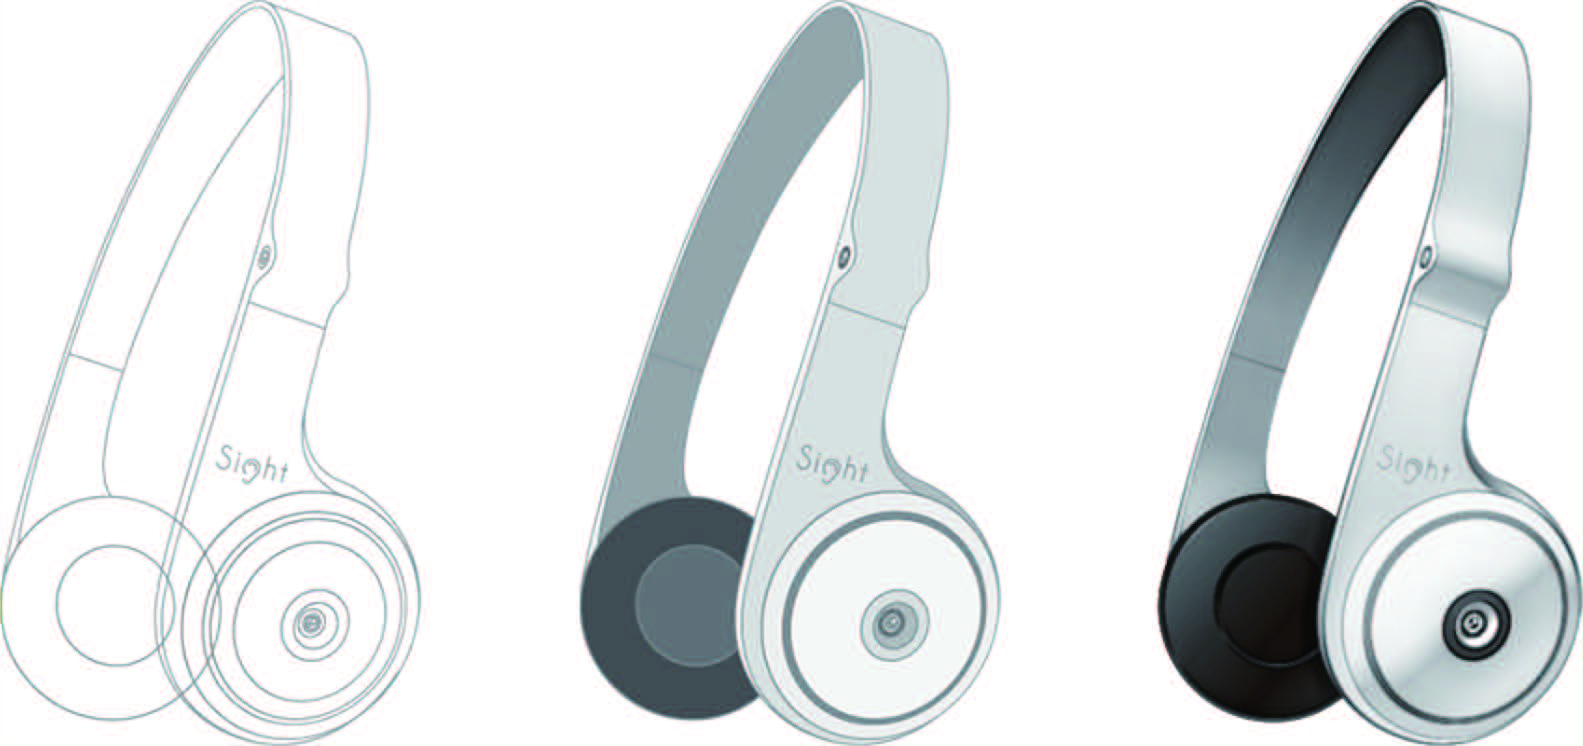
\includegraphics[height=40mm]{images/hardware/design_1.jpg}
\end{center}
\caption{プロジェクト考案当初のデザインスケッチ}
\label{fig:design_1}
\end{figure}

\heading{2015年8月}
内蔵するカメラやPC等の制限に囚われない理想的なプロダクトの3DCGイメージをモデリングソフト(fusion360)を用いて作成.
プロジェクトの目的は単なる生活向上ではなく「見る」という行為の追求に主眼を置いていた為,あえて目を覆い視覚をシャットダウンすることで,「目で見る」という既成概念を取り払うコンセプチュアルなデザインとした.(図.\ref{fig:design_2})


\begin{figure}[h]
\begin{center}
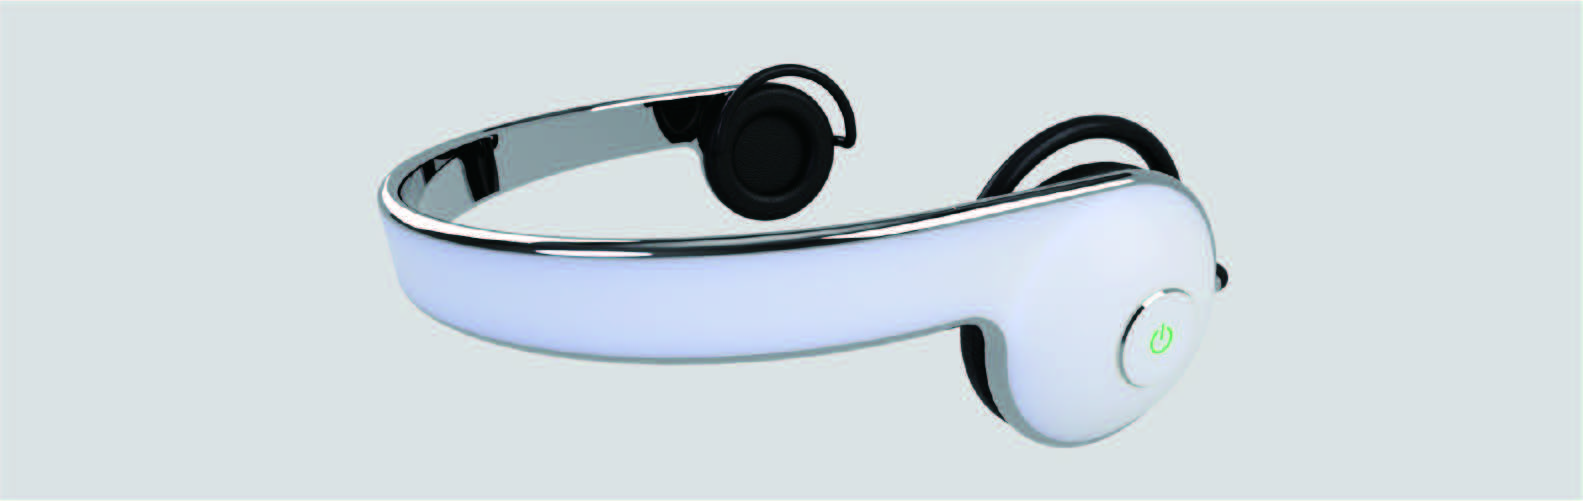
\includegraphics[height=40mm]{images/hardware/design_2.jpg}
\end{center}
\caption{コンセプチュアルデザイン}
\label{fig:design_2}
\end{figure}

\heading{2015年9月}
先のイメージを元に,Xtionやスピーカーを考慮した実用的なモデルをモデリング.(図.\ref{fig:design_3})

\begin{figure}[h]
\begin{center}
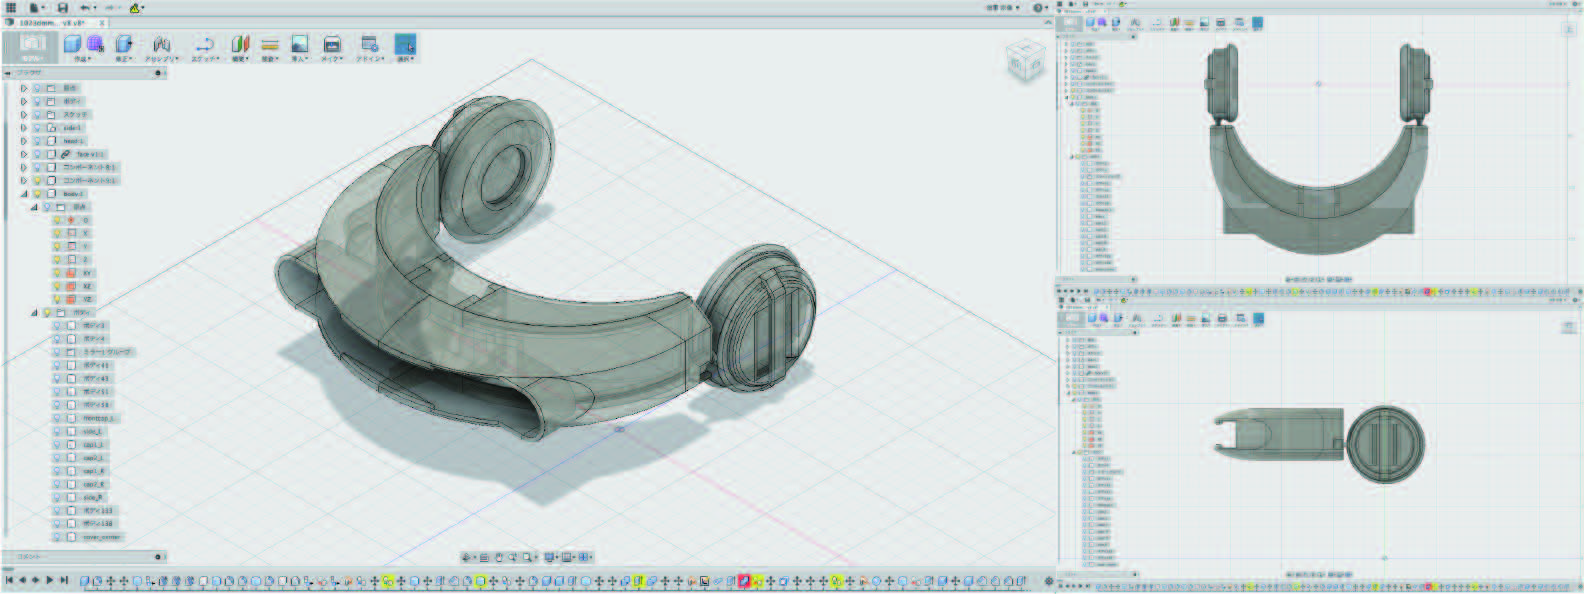
\includegraphics[height=45mm]{images/hardware/design_3.jpg}
\end{center}
\caption{モデリングの様子}
\label{fig:design_3}
\end{figure}

\heading{2015年10月}
DMM.makeAKIBAにて,制作したモデリングデータを3Dプリンタを用いて出力.Xtionやスピーカーの内蔵法,コード配線の設計,装着した際のフィット感等を実際に着けて確認し,修正を加えながらUXの改善に努めた.また,出力後はヤスリ掛けやパテによる穴埋め,下地となるサフの吹き付け,ガンスプレーを使用した塗装も行い,見た目としての完成度も向上させた.(図.\ref{fig:design_4})

\begin{figure}[h]
\begin{center}
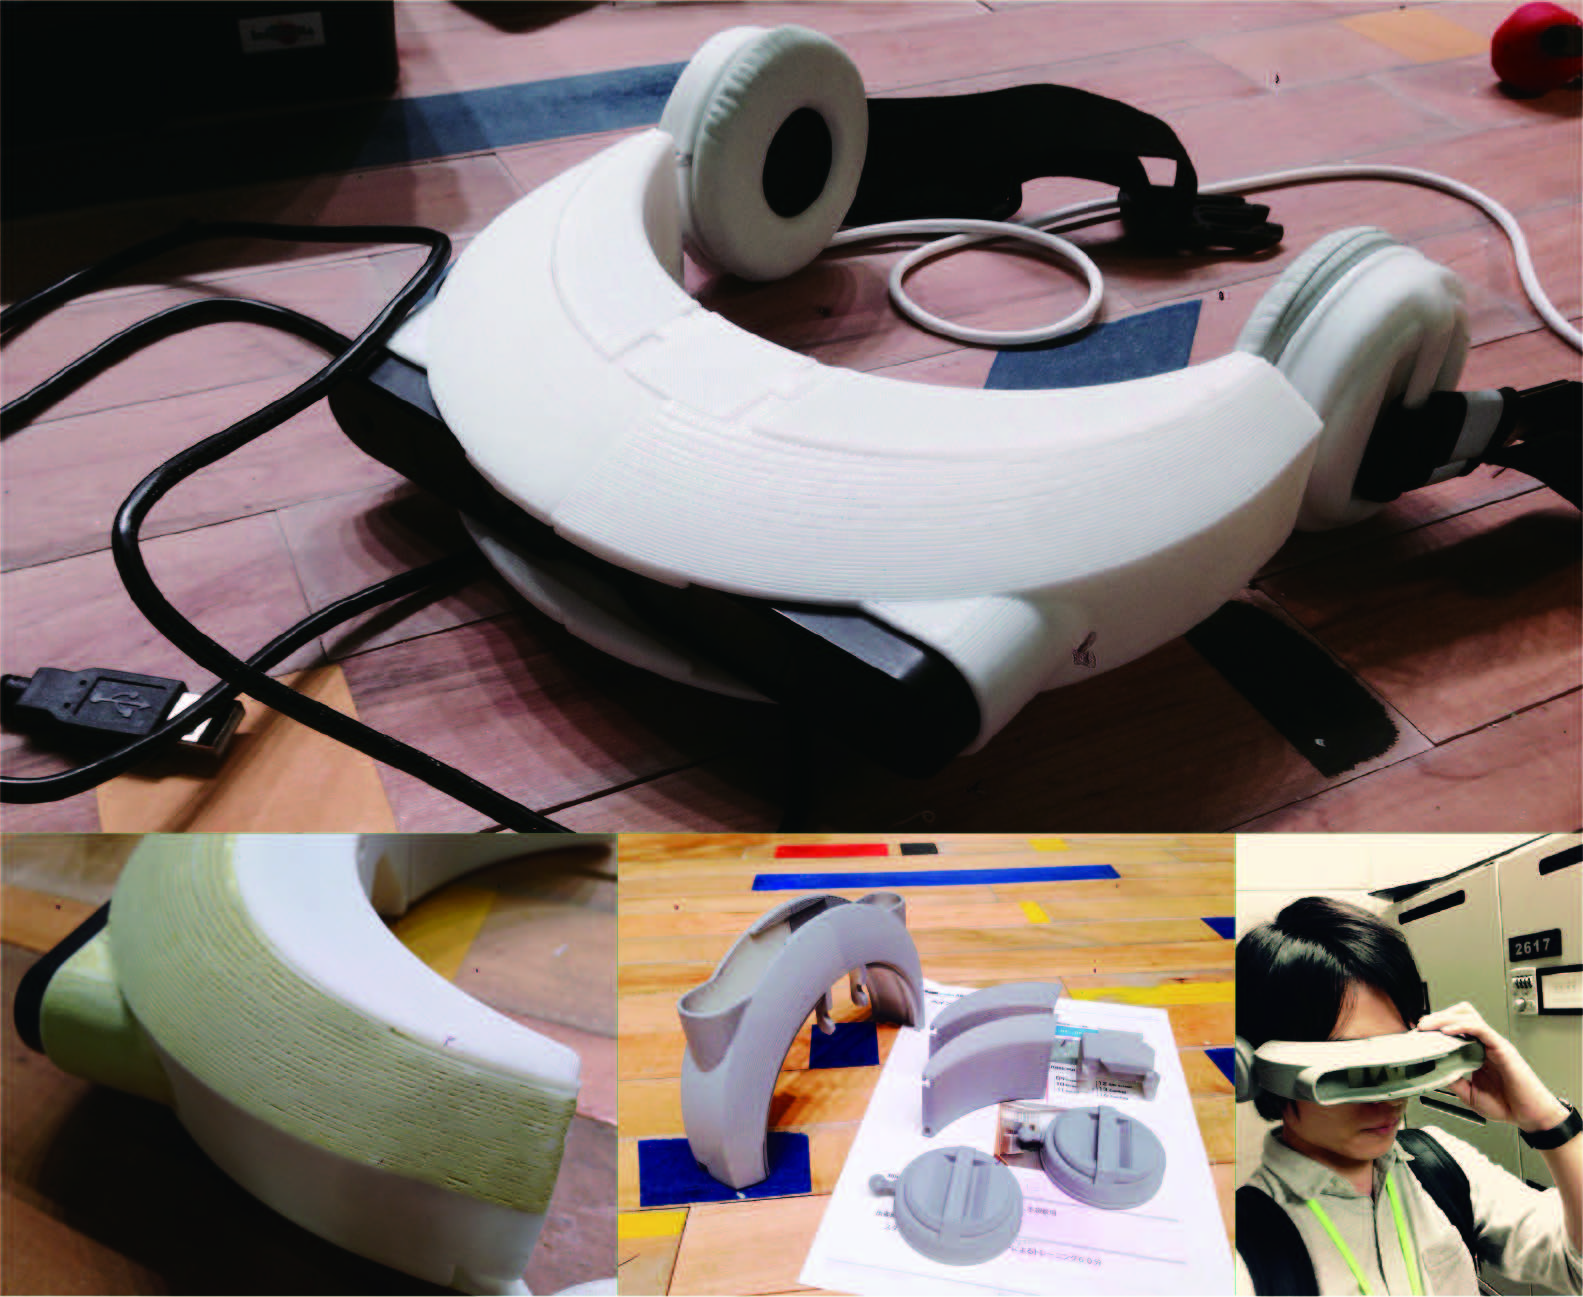
\includegraphics[height=75mm]{images/hardware/design_4.jpg}
\end{center}
\caption{3Dプリントの工程}
\label{fig:design_4}
\end{figure}

モデルは複数のパーツに分離しており,各々のパーツに凹凸を設けることで,度重なる試行錯誤の支障とならず,接着の一切不要.ハメ合わせの構造となっている凹凸の位置や形,幅についても何度も検証を繰り返し,より合理的で耐久性の強い組み合わせ方を試みた.(図.\ref{fig:design_5})

\begin{figure}[h]
\begin{center}
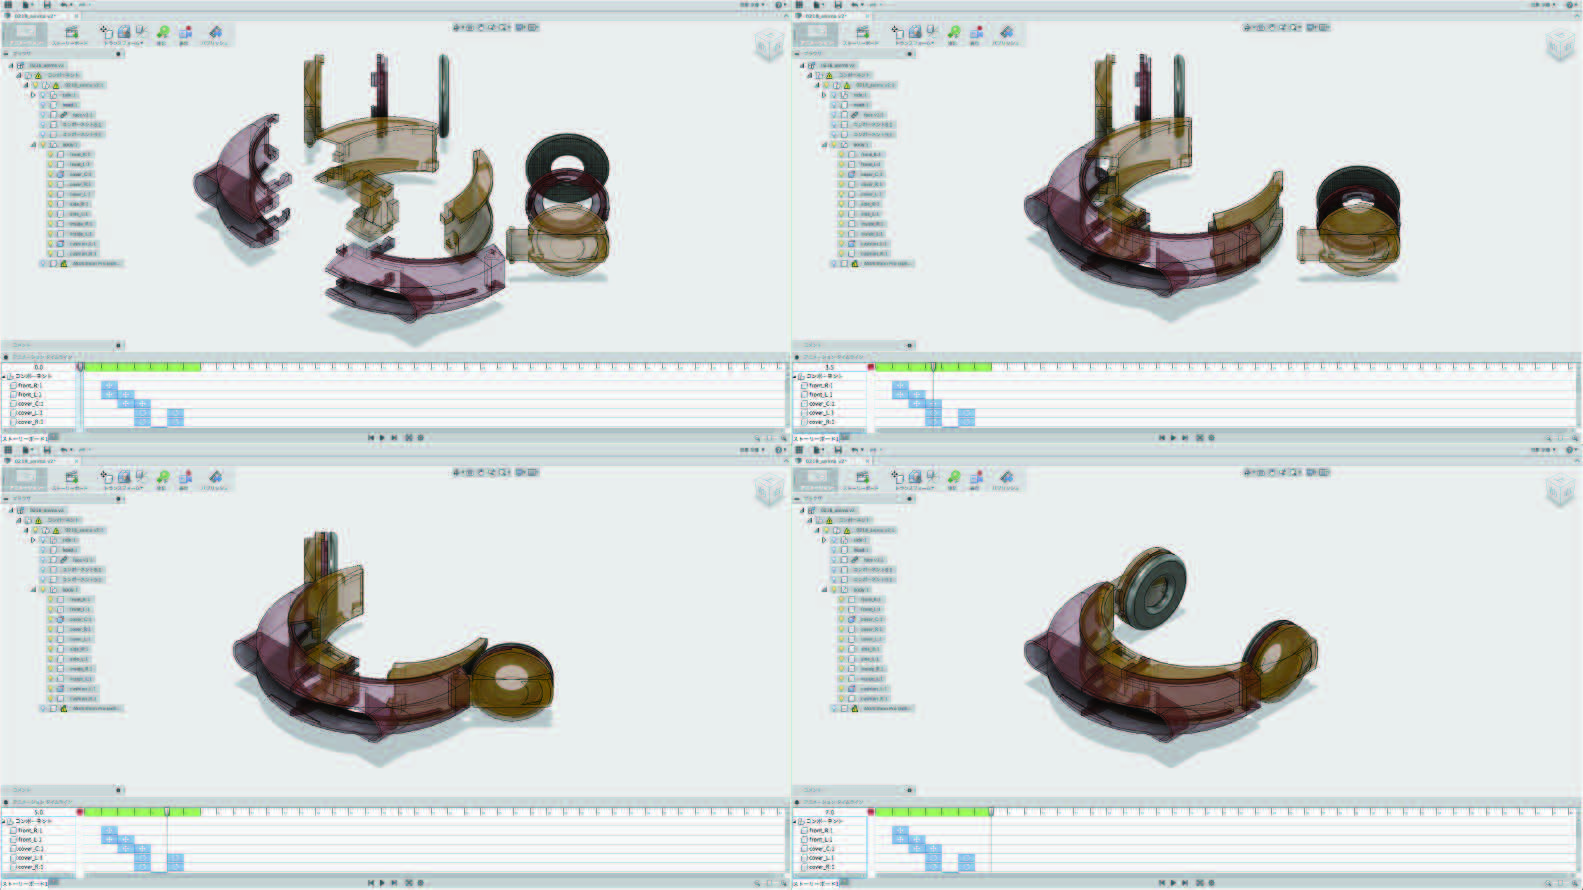
\includegraphics[height=60mm]{images/hardware/design_5.jpg}
\end{center}
\caption{はめ込み構造}
\label{fig:design_5}
\end{figure}

\heading{2016年1月}
以前のモデルで発覚した問題点を総ざらいし、改善バージョンをモデリングした。(図.\ref{fig:design_6})
\begin{itemize}
    \item イヤホンのジョイント部分の折れやすさ → デザイン性を保ちつつ幅や構造を見直
    \item 2バンド固定の緩さ→通し穴の位置を調整し、頭部とバンドの隙間をほぼゼロに
    \item スピーカー固定部分のネジ止めの摩耗 →はめ込み式のピースにし,ネジを排除
    \item 重さによるずり落ち → 頭頂部にもバンドを通し安定化
\end{itemize}

\begin{figure}[h]
\begin{center}
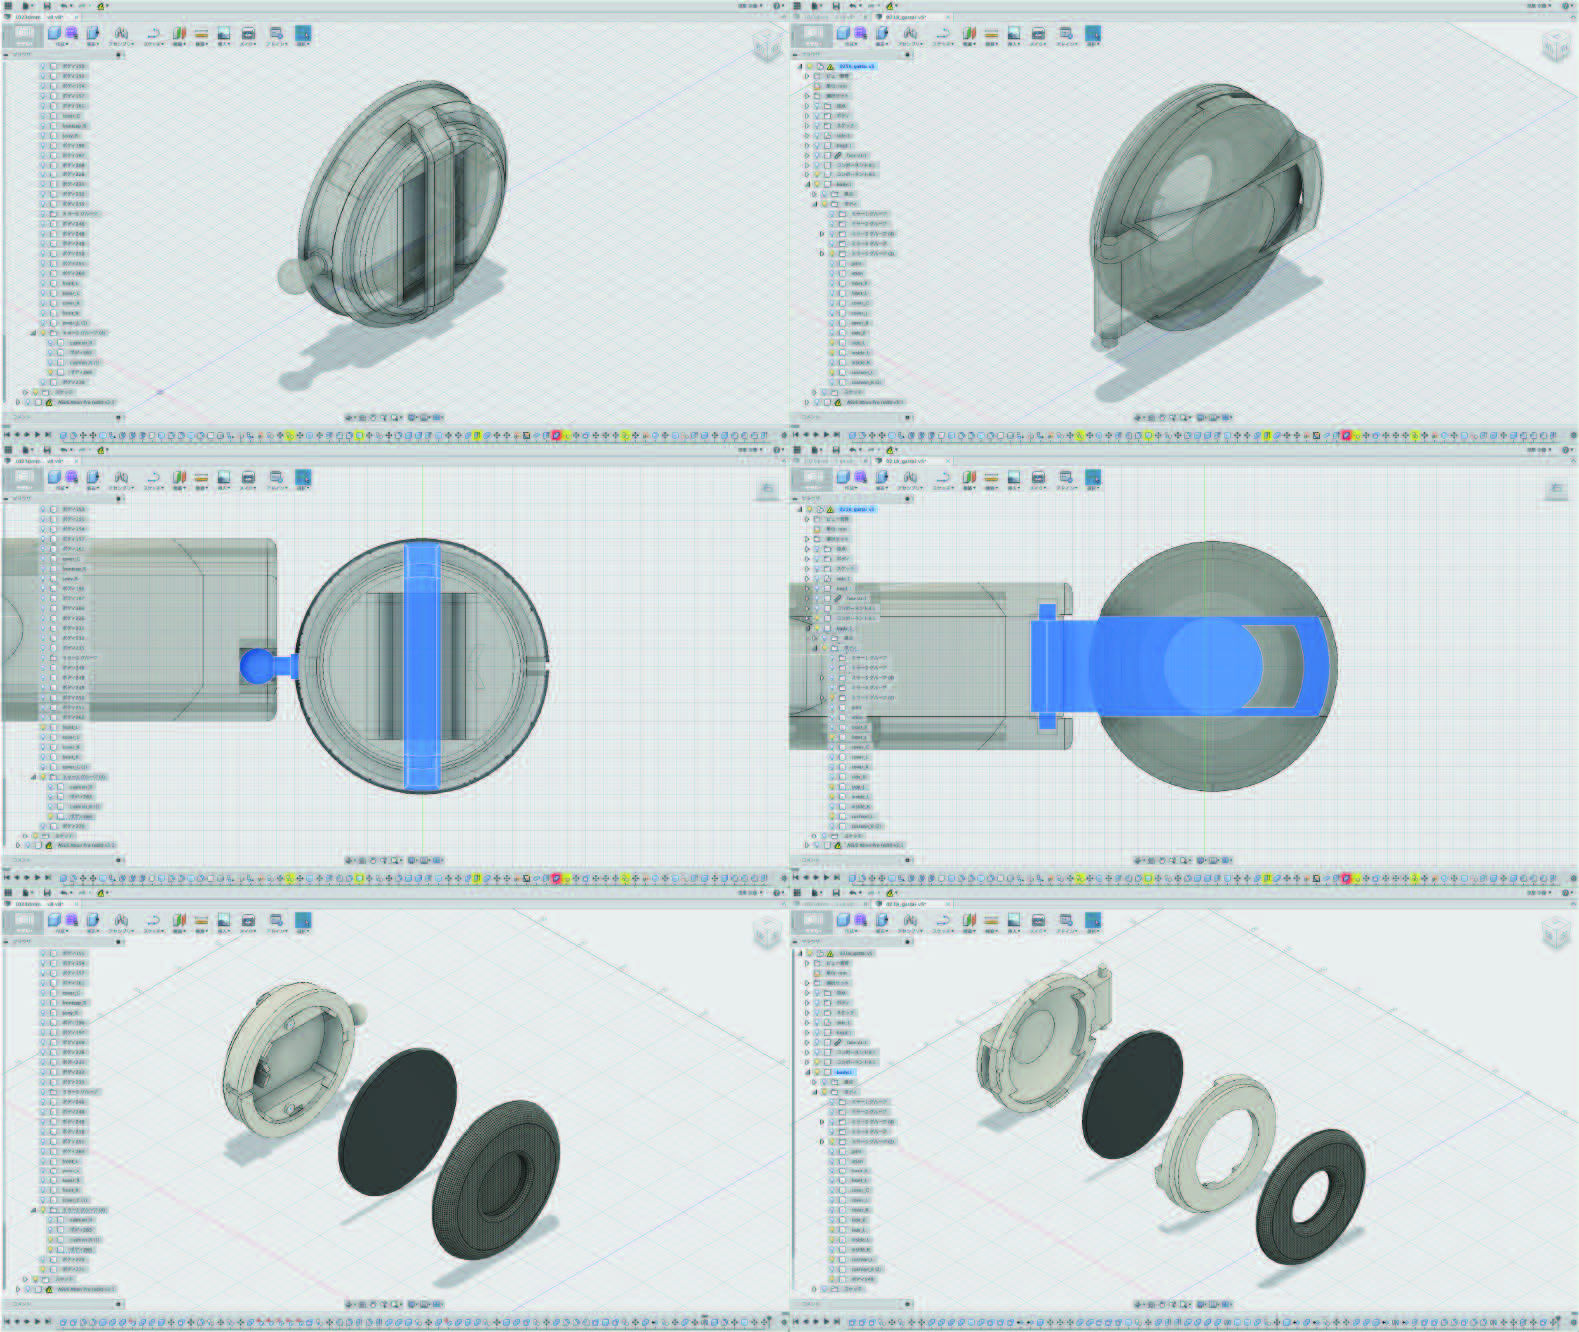
\includegraphics[height=70mm]{images/hardware/design_6.jpg}
\end{center}
\caption{デザインの改良}
\label{fig:design_6}
\end{figure}

\heading{2016年2月}
微調整を繰り返しながら最終成果報告会に向けた最終 ver を出力し、完成。(図.\ref{fig:design_7})
\begin{figure}[h]
\begin{center}
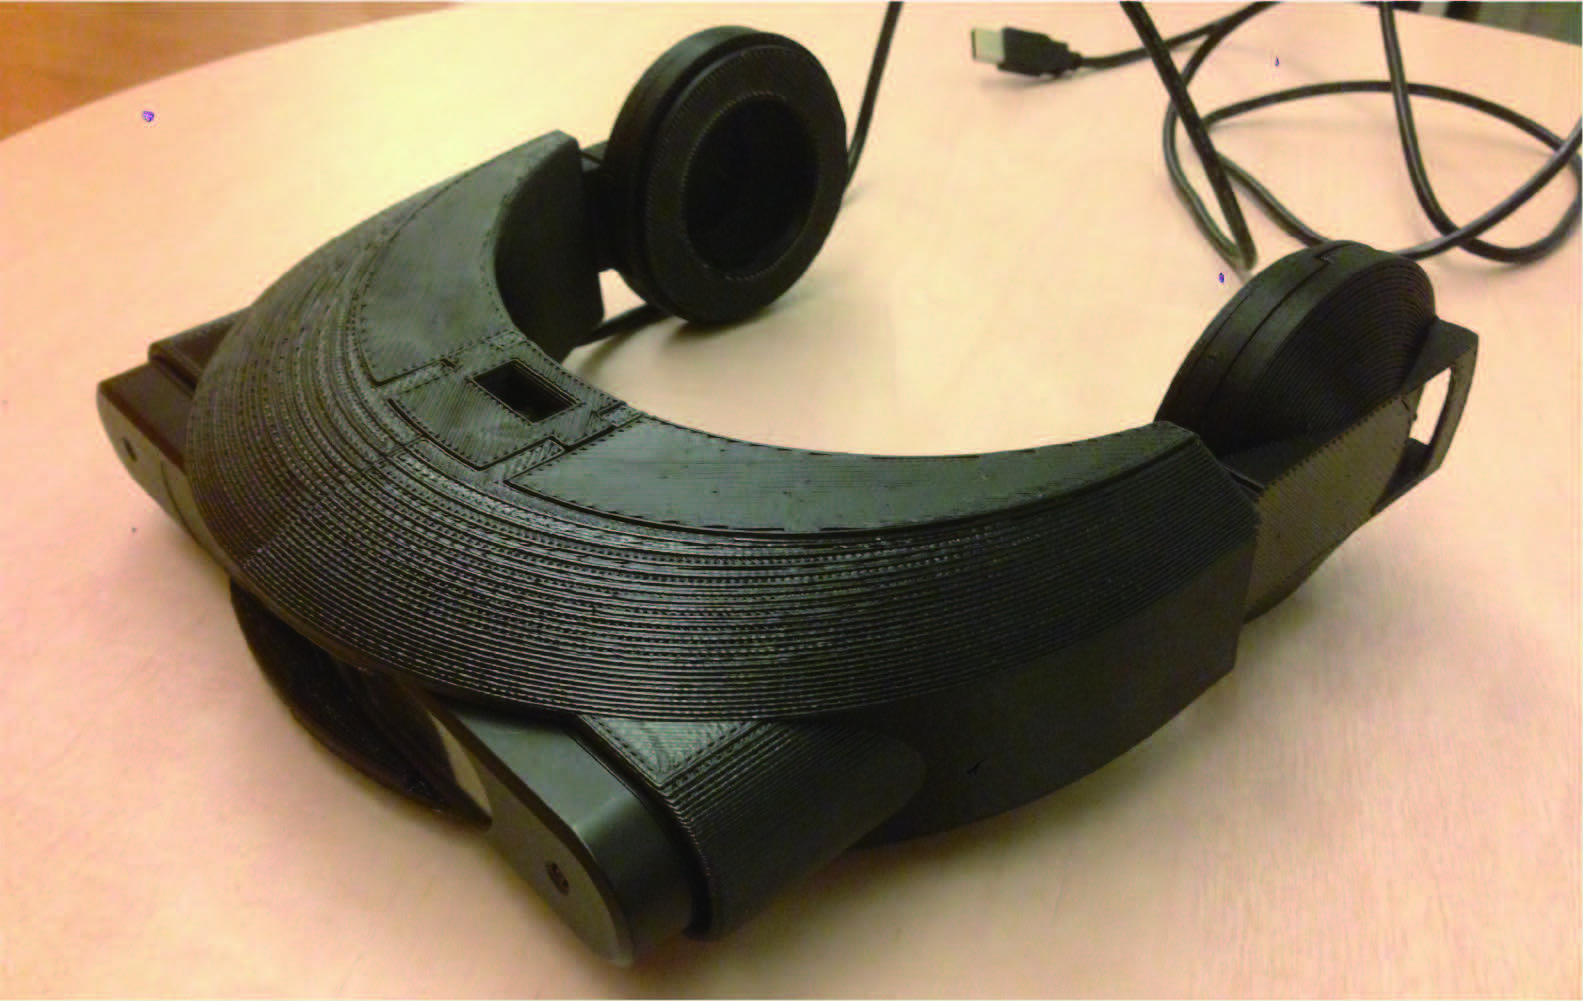
\includegraphics[height=60mm]{images/hardware/design_7.jpg}
\end{center}
\caption{最終バージョンのハードウェア}
\label{fig:design_7}
\end{figure}

\subsection{評価}
\subsubsection{タスク}
\subsubsection{ユーザスタディ}
\subsubsection{インタビュー}

